\section{Progettazione}
Qua ci sta una buona introduzione.

\subsection{Classificazione degli utenti}
Elenco puntato con i tipi di utenti e che cosa possono fare.
\\ Inserire tabella con username e password per lato admin

\subsection{Database}
spiegarlo \\
\begin{center}
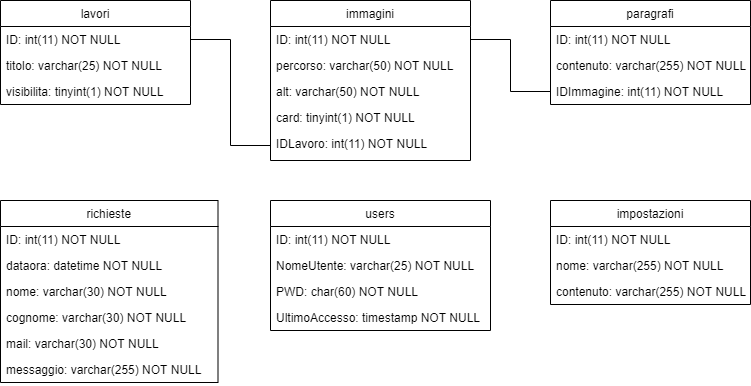
\includegraphics[scale = 0.5]{../latex/images/db.png}\\[1.5cm]
\end{center}

\subsection{Struttura dei contenuti}
dire che c'è lato clienti e lato admin.

\subsubsection{Lato cliente}
qualcosa qualcosa qualcosa qualcosa qualcosa qualcosa qualcosa qualcosa qualcosa qualcosa qualcosa qualcosa qualcosa qualcosa.\\\\
\textbf{Pagine}\\
qualcosa qualcosa qualcosa qualcosa	
	\begin{itemize}
		\item \textbf{Home} \\qualcosa qualcosa
		\item \textbf{Chi siamo}\\qualcosa qualcosa
		\item \textbf{Lavori}\\dire le pagine che lo compongono e cosa contengono
	 	\begin{itemize}
 			\item Matrimoni;\\	qualcosa qualcosa 
	 		\item Lauree;\\	qualcosa qualcosa 
 			\item Funerali;\\	qualcosa qualcosa
 			\item ...; 		 		
	 	\end{itemize}
	 	\item \textbf{Contatti}\\qualcosa qualcosa\\
 	\end{itemize}
\textbf{Parti fondamentali -> troviamoci un sinonimo}\\ 
	qualcosa qualcosa qualcosa
	\begin{itemize}
		\item \textbf{Header}\\qualcosa qualcosa
		\item \textbf{Breadcrumb}\\qualcosa qualcosa
		\item \textbf{Footer}\\qualcosa qualcosa
 	\end{itemize}
 		
\subsubsection{Lato Admin}
- discorso login
- discorso session\\\\
\textbf{Pagine}\\ qualcosa qualcosa qualcosa
	\begin{itemize}
		\item \textbf{Dashboard};\\qualcosa qualcosa
		\item \textbf{Gestione richieste};\\qualcosa qualcosa
		\item \textbf{Gestione categorie};\\dire le pagine che lo compongono e come funziona il tutto
	 	\begin{itemize}
 			\item Aggiungi categoria;\\qualcosa qualcosa
 			\item Modifica categoria;\\qualcosa qualcosa
 			\item Elimina categoria;\\qualcosa qualcosa
	 	\end{itemize}
 	\item \textbf{Gestione utenti}\\qualcosa qualcosa qualcosa
 	\item \textbf{Logout}\\qualcosa qualcosa qualcosa\\
 	\end{itemize}
\textbf{Parti fondamentali -> troviamoci un sinonimo} \\
\begin{itemize}
	\item \textbf{Breadcrumb}\\	qualcosa qualcosa qualcosa
	\item \textbf{Funzionamento PHP}\\	DbConnection ecc.
\end{itemize}